% This is LLNCS.DEM the demonstration file of
% the LaTeX macro package from Springer-Verlag
% for Lecture Notes in Computer Science,
% version 2.3 for LaTeX2e
%
\documentclass{llncs}
%
\usepackage{makeidx}  % allows for indexgeneration
\usepackage{graphicx}
\usepackage{multicol} 
\usepackage{subfigure}
\usepackage{mathptmx} % use Times fonts if available on your TeX system
\usepackage{setspace}
%
\begin{document}
\title{Decentralized Communications for Self-regulated Division of Labour in Robot Society
\thanks{This research has been funded by the Engineering and Physical Sciences Research Council (EPSRC), UK, grant reference EP/E061915/1.}
}
%\subtitle{Do you have a subtitle?\\ If so, write it here}
\titlerunning{Decentralized Communications for Self-regulated Division of Labour in Robot Society} % if too long for running head
\author{Md Omar Faruque Sarker \and
	Torbjorn Dahl %etc.
}
%\authorrunning{Short form of author list} % if too long for running head
\institute{ 
	Robotic Intelligence Lab,
	Newport Business School\\
	University of Wales, Newport,
	Allt-yr-yn Campus\\ Allt-yr-yn Avenue, Newport, NP205XR, UK\\
	\email{Mdomarfaruque.Sarker@newport.ac.uk\\ 
	Torbjorn.Dahl@newport.ac.uk}
}
%\date{Received: / /  Accepted:  /  /  }
% The correct dates will be entered by the editor
\maketitle
\begin{abstract}
Distributed local communication is one of the essential means by which various social insects achieve their self-regulatory division of labour. Unlike centralized static communication, this communication mode enables individuals to respond to local changes more quickly and it generally produces steady-state convergence of self-regulated division of labour (DoL) in social insects. However, realizing this kind of communication in a distributed multi-robot system (DMRS) is not as straight forward as a centralized one. From a robot controller's point of view, it is not easy to determine how often or how much dynamic peer-to-peer (P2P) communication  is needed to maintain system's convergence of division of labour. In this paper, we address these questions: first by describing our reference centralized communication based DMRS that shows a steady-state convergence of self-regulated DoL. Then we compare this system with our two local communication based DMRS with two different communication radii. All experiments on these systems  have been done with 16 physical E-puck robots in an area of about 4$m^2$. Results from these experiments suggest that faster and stable convergence can be obtained by setting a smaller P2P communication radius where a robot locally exchanges signals with a minimum number of its closest peers.
%\keywords{First keyword \and Second keyword \and More}
%% \PACS{PACS code1 \and PACS code2 \and more}
%% \subclass{MSC code1 \and MSC code2 \and more}
\end{abstract}
\addtolength{\parskip}{-3.5mm}
\section{Introduction}
\label{sec:intro}
\vspace{2mm}
Multi-agent task allocation or division of labour (DoL) is a challenging research issue in the field of multi-agent and multi-robot systems e.g., swarm robotics \cite{RefSwarm}. In order to address this issue, existing approaches e.g., predefined (off-line) and emergent (real-time) task-allocation, fail to scale well with large number of agents. Typically, increased communication interference and decreased bandwidth among agents are major causes of this problem. Unlike the swarm robotic approach, which is inspired by biological systems alone and commonly aims for minimal intelligence agents, we propose to solve DoL in multi-agents based on a set of observed generic rules of DoL from biological and human social systems. These bottom-up rules describe the phenomena of self-regulated DoL in terms of attractive fields between agents and tasks. The concrete form of these rules, termed as \textit{attractive filed model} (AFM) \cite{RefElsa}, offers a scalable solution to the above DoL problem. Unlike having strong dependence to communication mediums by most of the existing approaches, our model states that self-regulatory DoL can be established by AFM without maintaining a strong form of on-line communication. 

\vspace{4mm}
We intend to investigate the performance of three different communication strategies for self-regulated DoL among larger robot teams: global, local and stigmergic. The global and local forms of communications typically resemble to message broadcast and peer-to-peer (P2P) communications respectively. In stigmergic communication mode, individuals leave information in the environment e.g., pheromone dropping of ants. We intend to find out the convergence of self-regulated DoL in the above modes irrespective of size of robot teams.
%
%\addtolength{\topskip}{-15mm} 
\section{Modeling}
\label{sec:model}
\vspace{2mm}
According to AFM, the strength of field of a task (j) of a robot (i) or stimuli of an attractive filed $S_{j}^{i}$ can be estimated using Eq. \ref{eqn1} .
\addtolength{\abovedisplayskip}{-10mm} 
\begin{scriptsize}
\begin{multicols}{2} 
\begin{equation}
S_{j}^{i} = tanh\{\frac{k_{j}^{i}}{d+\delta } \phi _{j}\}
\label{eqn1}
\end{equation}
\vspace*{0.25cm}
\begin{equation}
P_{j}^{i} = \frac{S_{j}^{i}}{\sum_{j}^{}S_{j}^{i}}
\label{eqn2}
\end{equation}
\end{multicols}
\end{scriptsize}
%\addtolength{\belowdisplayskip}{-1mm} 
\vspace{2mm}
This stimuli of a particular task depends on agent's spatial distance to that task (d), level of sensitization of that agent to that task ($k_{j}^{i}$) and perceived urgency of that task ($\phi _{j}$). In each discrete time-step $k_{j}^{i}$ and $\phi _{j}$ change according to the properties of a target system. Using Eq. \ref{eqn2} the probability of selecting each task has been determined by a probabilistic method.
%\begin{spacing}{0.5}
\addtolength{\floatsep}{-25mm}
\begin{figure}[ht]
\begin{minipage}[b]{0.55\linewidth}
\centering
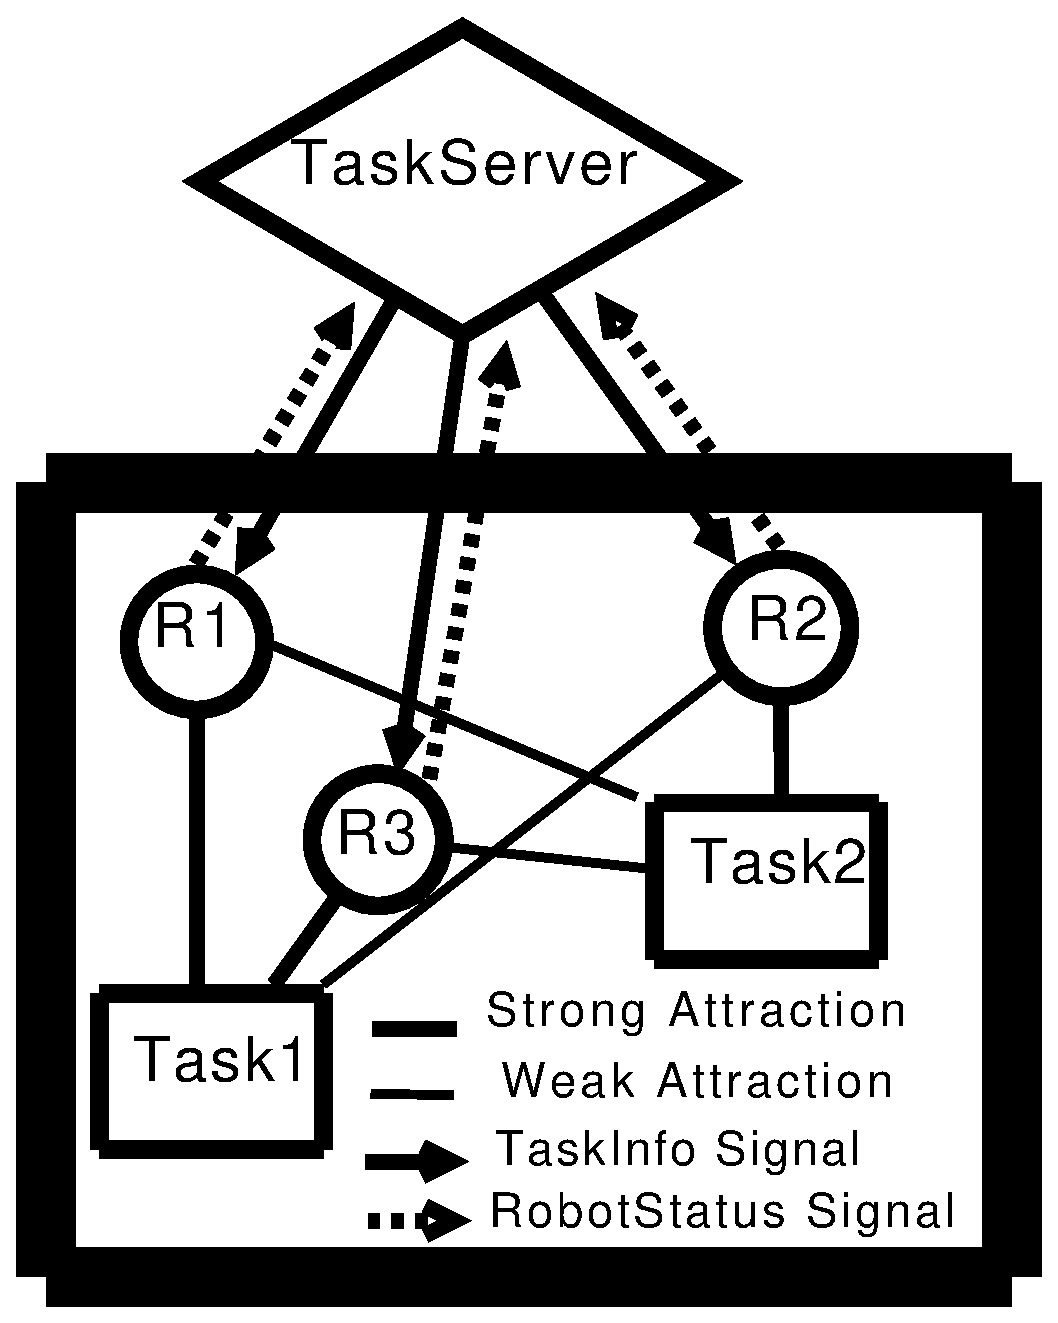
\includegraphics[height=6cm, angle=0]{../dia-files/CentralizedComm.eps}
% figure caption is below the figure
\caption{Centralized communication model}
\label{fig:1} % Give a unique label
\end{minipage}
%\hspace{0.5cm}
\begin{minipage}[b]{0.45\linewidth}
\centering
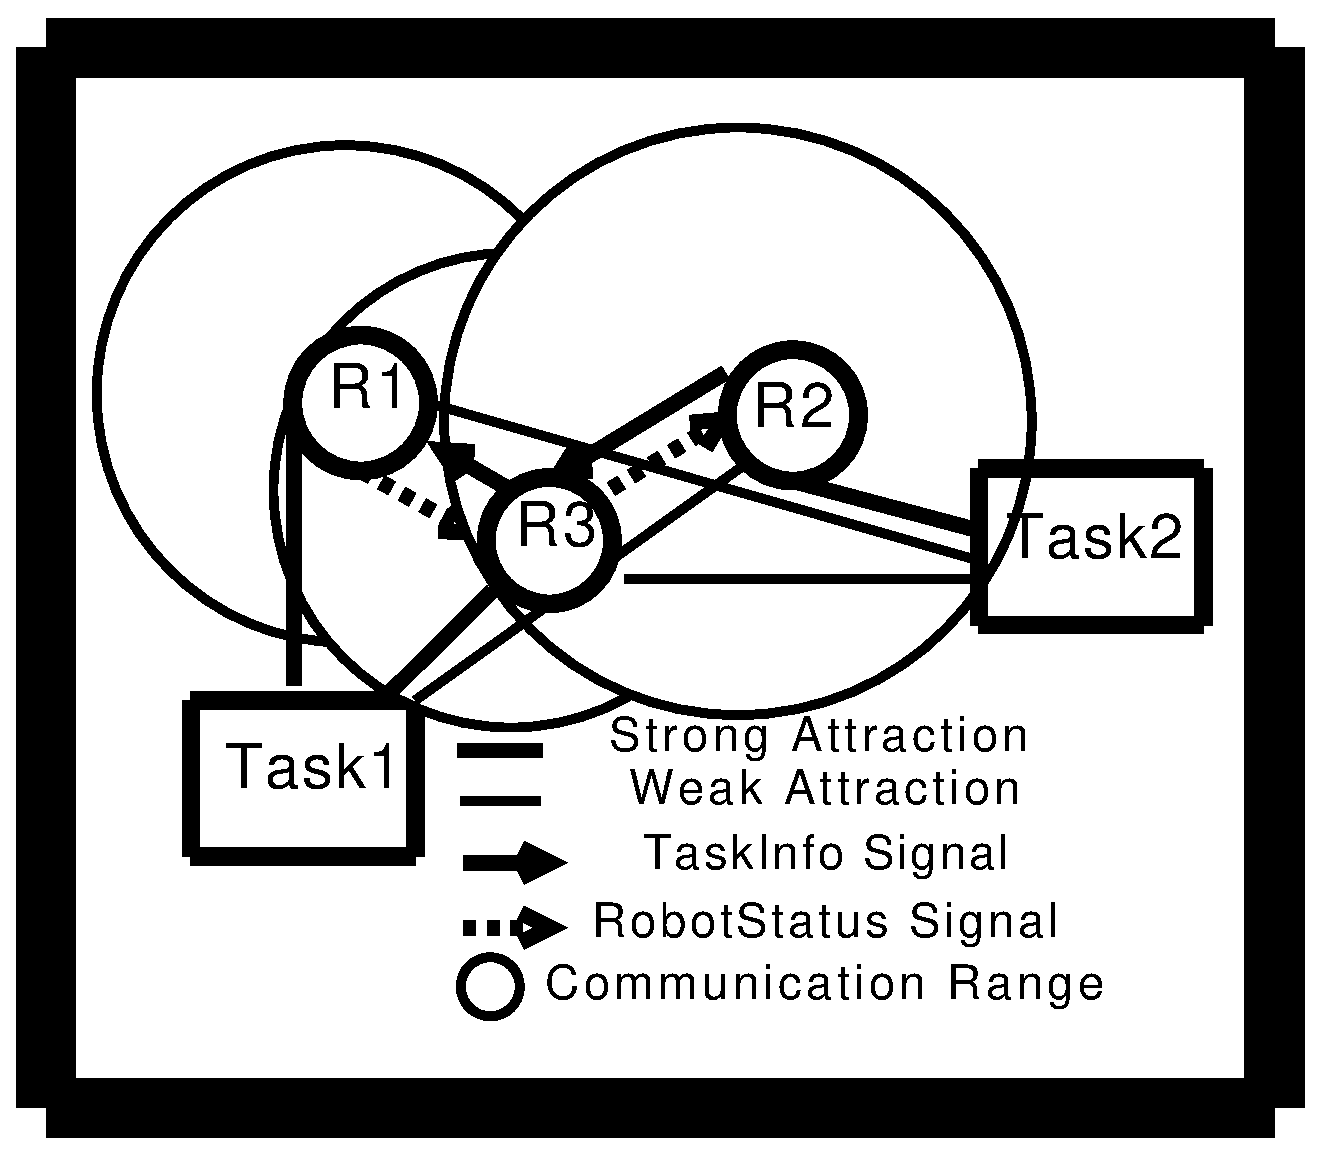
\includegraphics[height=4cm, angle=0]{../dia-files/LocalComm.eps}
% figure caption is below the figure
%\vspace*{0.20cm}
\caption{Local communication model}
\label{fig:2} % Give a unique label
\end{minipage}
\end{figure}
%\addtolength{\belowcaptionskip}{-15mm}
%\end{spacing}
As shown in Fig. \ref{fig:1} AFM has been implemented in our multi-robot system consisting of a group of E-puck robots, a Prosilica Gigabyte Ethernet(GigE) GC4900C camera and a Dell Precision server grade PC. The overhead camera captures the image of an experiment area of about 3.6m x 3.2m and sends the image frame to an open-source tracking platform SwisTrack (http://swistrack.sf.net). SwisTrack detects the robot id and pose based on the location of robot markers in the image. This information has been passed into AFM Main-Loop component that portrays circular tasks in the image and stores tasks and robot pose info into a shared memory of server PC. Each physical robot is controlled by an identical client program that relies on Player robot control platform (http://playerstage.sf.net) to transfer commands to/from robot's firmware via Bluetooth wireless link. This client program retrieves task info and robot's pose from shared memory in real-time.
%\addtolength{\topskip}{-15mm} 
% 
\section{Experiment Design}
\label{sec:expt-design}

\section{Implementation}
\label{sec:impl}

\section{Results and Discussions}
\label{sec:results}
In our first tier of experiments, we emulated global mode communication by broadcasting task and pose messages to robot clients. Initially we set each task urgency to 0.5. After a set time intervals AFM Main-Loop checks the number of robots working on each task. If no robots works on a task, its urgency has been increased by a small amount of 0.01, otherwise urgency has been decreased by same amount. Robots use these task urgency and pose message broadcasts in calculating task stimulus.

\begin{figure}
\begin{minipage}[t]{0.5\linewidth}
\centering
\includegraphics[height=5cm,  angle=0]
%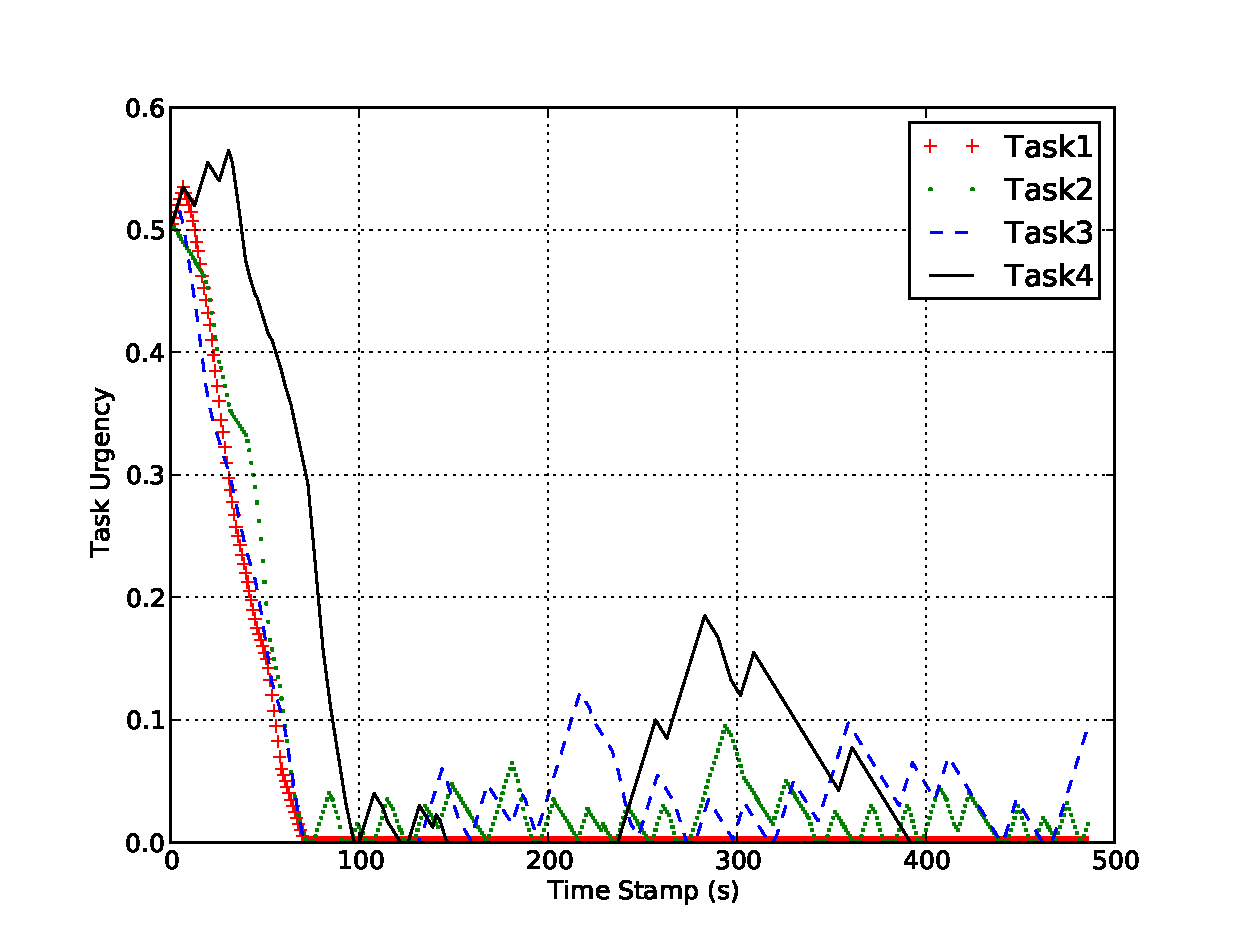
\includegraphics[width=10cm, angle=0]
{images/global/GlobalPlotUrgencyLog-2010Feb18-151600-clear.eps}
 %figure caption is below the figure
\caption{Task urgency changes in centralized communication model}
\label{fig:1} % Give a unique label
\end{minipage}
\hspace{0.5cm}
\begin{minipage}[t]{0.5\linewidth}
\centering
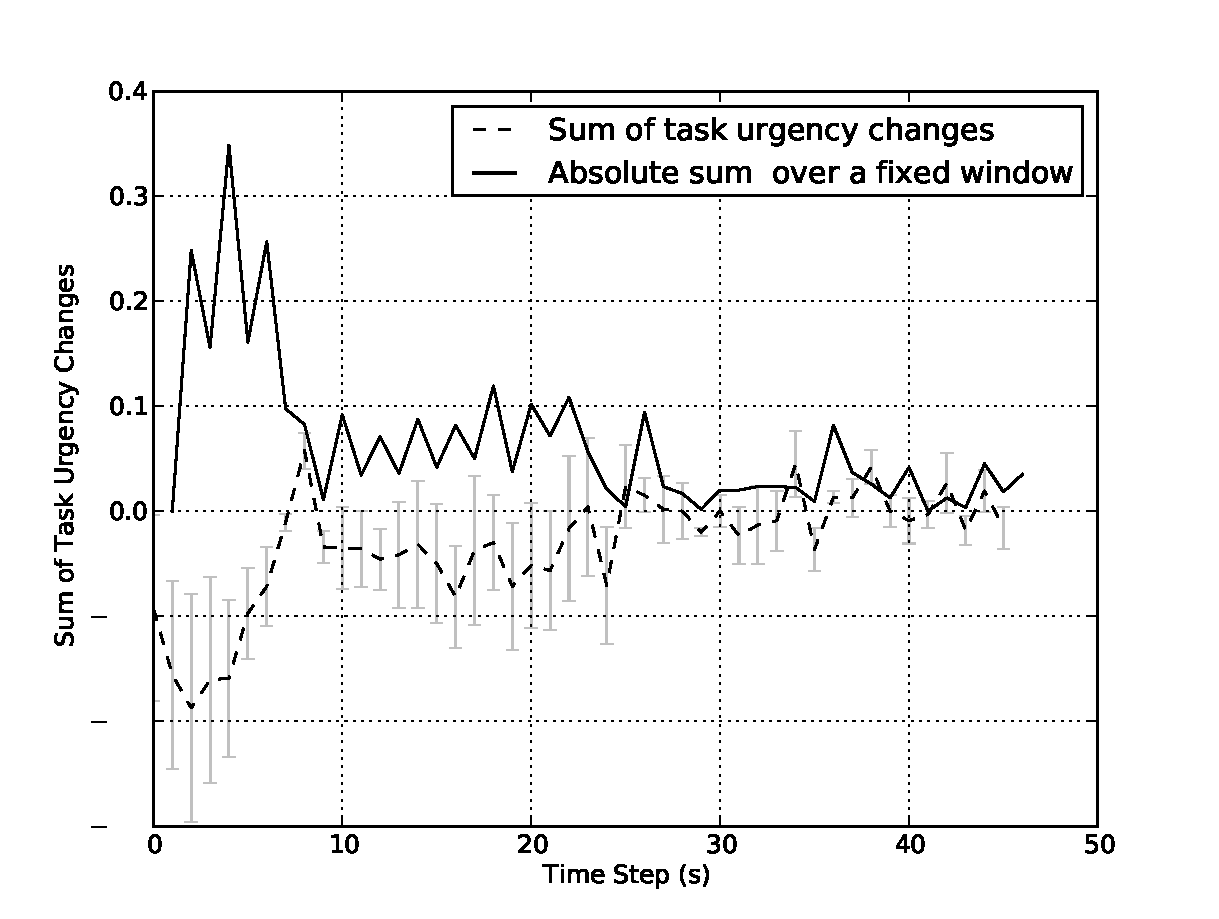
\includegraphics[height=5cm, angle=0]{images/global/TaskUrgencyConvergence-step2-th-p1.eps}
% figure caption is below the figure
%\vspace*{0.20cm}
\caption{Task urgency convergence in centralized communication model}
\label{fig:2} % Give a unique label
\end{minipage}
\end{figure}
%\vspace*{1cm}



\section{Conclusion and Future works}
\label{sec:conc}
 Initially robots sensitization to all tasks has been set to 0.1. We set a simple learning rule for sensitization so that if a robot selects a task in Nth step and if the same task has been selected in next (N+1)th step, sensitization of that task (j) for that robot (i) has been increased by a learning coefficient L and at the same time sensitization of other tasks has been decreased by a forgetting coefficient F. This ensures flexibility and concurrency of robots to switch from one task to another.
%
%The global mode experiments have established a base line of self-regulated DoL using broadcast communication strategy. 
As shown in Fig. \ref{fig:2} task urgency varies as robots switch among tasks. %and when 6 robots works in 3 tasks we find a convergence of DoL to near zero. 
%
After some time, when a few working robots have intentionally been removed from the experiment, urgency of some unattended tasks have been increased immediately. When this removed robots return to the experiment urgency of all task again converges to zero. This shows the robustness of AFM for self-regulated DoL. %It relied on decentralized control strategies based on a set of generic rules.
%
Our future works include iterating above experiments using local and stigmergic communication modes with a larger group of robots (about 40). %The goal is to find out necessary ingredients to reach similar level of self-regulated DoL with varying team sizes. 
%\begin{acknowledgements}
%If you'd like to thank anyone, place your comments here
%and remove the percent signs.
%\end{acknowledgements}
% BibTeX users please use one of
%\bibliographystyle{spbasic} % basic style, author-year citations
%\bibliographystyle{spmpsci} % mathematics and physical sciences
%\bibliographystyle{spphys} % APS-like style for physics
%\bibliography{} % name your BibTeX data base
% Non-BibTeX users please use
\begin{thebibliography}{}
%
% and use \bibitem to create references. Consult the Instructions
% for authors for reference list style.
%
\bibitem{RefSwarm}
% Format for Journal Reference
Erol Sahin and Alan Winfield, Special issue on swarm robotics, Swarm Intelligence, Vol 2, 69-72 (2008)
% Format for books
\bibitem{RefElsa}
Elsa Arcaute \textit{et} al., Division of labour in ant colonies in terms of attractive fields, Ecological Complexity, Elsevier (2008)
% etc
\end{thebibliography}
%
\end{document}
